\subsection{Gebruikers}

Geregistreerde gebruikers kunnen bepaalde acties uitvoeren op de website waar anonieme gebruikers dat niet kunnen. 
De onderstaande screenshot toont de 'Gebruikers interface' met al haar opties en mogelijkheden.

\bigskip

\begin{center}
	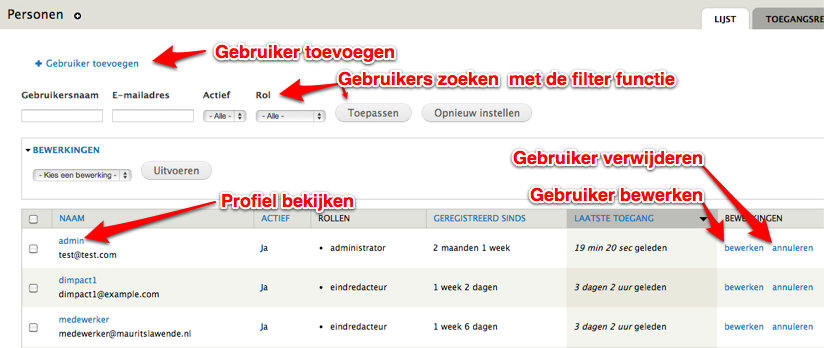
\includegraphics[width=\textwidth]{img/gebruikers1.png}
\end{center}

\subsubsection{Gebruikers toevoegen}

Gebruikers kunnen aangemaakt worden via de frontend(registratie) en via de backend. Deze paragraaf beschrijft hoe je manueel gebruikers kunt toevoegen via de backend. 

Ga naar 'Personen' en klik vervolgens op 'Gebruiker toevoegen', of ga direct naar \drupalpath{admin/people/create}.

Vul alle verplichte velden in en selecteer eventueel welke rol de gebruiker dient te hebben.
Klik onderaan de pagina op 'Nieuw account aanmaken' om de gebruiker toe te voegen.

\subsubsection{Gebruikers bewerken}

Ga naar 'Personen' en klik bij de betreffende gebruiker in de meest rechter kolom op 'bewerken' om het account te gaan bewerken. 
Bewerk het account naar wens en klik vervolgens onderdaan de pagina op de knop 'Opslaan' om de wijzigingen op te slaan.

\subsubsection{Gebruikers verwijderen}

Ongewenste gebruikers accounts kunnen verwijderd worden uit de database; de volgende manier is de meest makkelijke:
Ga naar 'Personen' en kruis in de meest linker kolom aan welke gebruiker je wilt gaan verwijderen, het is mogelijk om meerdere gebruikers tegelijk te verwijderen. Selecteer bij 'Update-instellingen' welke actie je wilt gaan uitvoeren, klik in dit geval op 'Geselecteerde gebruikersaccounts annuleren'. Om de gebruiker(s) daadwerkelijk te verwijderen uit de database klik je op de knop 'Bijwerken'. Let op: deze actie is permanent en kan niet (zomaar) ongedaan worden gemaakt. 

